\section{Služby komunikačních systémů -- obecný rozbor, signalizační systém SS7, Telecommunication Management Network -- TMN, telekomunikační služby z pohledu ekonomiky.}

\subsection{Služby komunikačních systémů}
Služby komunikačních systémů jsou funkce poskytované přes komunikační sítě a zařízení, které umožňují uživatelům komunikovat a vyměňovat informace. Patří sem hlasové a datové služby, SMS a MMS, videohovory, VoIP, mobilní služby a další. Jejich cílem je usnadnit komunikaci a výměnu informací mezi uživateli.

\subsection{Telekomunikační služby}
Telekomunikační služby přenášejí informace pomocí signálů a mohou obsahovat text, zvuk nebo obraz. Telekomunikační síť je systém, který umožňuje výměnu dat a spojení mezi koncovými zařízeními. Vývoj telekomunikačních služeb začal v 60. letech a dnes existují globální sítě, jako je internet. Síťová architektura a vrstevnatá struktura definují způsob komunikace a řízení v telekomunikačních systémech. Protokoly slouží k výměně údajů mezi komunikujícími prvky a dodržování pravidel a procedur. Přenosové systémy sítí jsou standardizovány pro zajištění vyšší propustnosti a spolehlivosti sítí.

Přístupové sítě -- metalické (telefonní), datové (xDSL, ISDN), optické (PON), bezdrátové (mobilní GSM)

\subsubsection{Základní prvky}
\begin{description}
    \item[vysílač] Příprava, zpracování a vložení informace do komunikačního kanálu pomocí signálu.
    \item[přenosové médium] Prvky vytvářející přenosové prostředí pro přenos informace v požadované podobě signálu -- elektromagnetické, rádiové, kabelové, optické.
    \item[přijímač] Příjem informace, signálu z přenosového prostředí a jeho zpracování pro předání cílovému subjektu.
\end{description}

\subsubsection{Kategorizace}
\begin{itemize}
    \item Podle typu zpracování informace:
          \begin{description}
              \item[Analogové] Telefonní síť, terestiální analogové vysílání atp. (v dnešní době postupně zanikající služby, nahrazované digitálními technologiemi).
              \item[Digitální] Datová síť -- většina dnes nabízených služeb.
          \end{description}
    \item Podle regulace:
          \begin{description}
              \item[Rezervované služby] Jedná se o služby telefonního charakteru.
              \item[Oblasti regulované licenčními podmínkami] Televizní a rádiové vysílání, mobilní komunikace.
              \item[Oblasti volného působení za dodržení norem a předpisů] Služby uživatelského charakteru.
          \end{description}
    \item Podle potřeb uživatelů:
          \begin{description}
              \item[Základní a rozšířené telefonní služby] Telefonní hovory, datové služby ISDN, doplňkové služby ke zdokonalení základní služby, jako je například přenos telefonního čísla, volání na účet volaného, roamingové služby, textové a hlasové zprávy apod.
              \item[Telematické datové služby] Využívající stávající telekomunikační sítě v infrastruktuře dopravy v ČR.
              \item[Multimediální datové služby] IPTV internetové televizní vysílání, VoIP -- internetová telefonie, ISP -- poskytování služeb internetu a podobně, jsou kladeny vyšší nároky na přenosová média z hlediska zpracování a rychlosti doručení informace.
          \end{description}
    \item Podle počtu současně komunikujících účastníků:
          \begin{description}
              \item[Bod-bod: point to point] Komunikace pouze dvou uživatelů, bodů, na přenosovém médiu.
              \item[Bod-více bodů: point to multipoint] (Centralizované) komunikace jednoho uživatele s více, TV, IPTV, rozšířené telefonní služby a rádiové vysílání, některé služby ISP.
              \item[Více bodů-více bodů: multipoint to multipoint] (Decentralizované) -- videokonference, sdílení sítí a výpočetních prostředků na síti, P2P, PC hry a podobně.
          \end{description}
    \item Podle dosažitelnosti služeb:
          \begin{description}
              \item[Pevné] Digitální integrované služby ISDN, služby asynchronních sítí ATM, služby sítí LAN, služby internetového charakteru.
              \item[Mobilní] Služby bezdrátových paketových sítí, služby GSM standardů.
          \end{description}
\end{itemize}

\subsection{Signaling System Number 7 (SS7)}
Signalizační systém SS7 (Signaling System Number 7) je sada signalizačních protokolů používaných v mobilních telefonních sítích, pozemních digitálních telefonních sítích a pro mezi-ústřednovou signalizaci. Úkolem signalizačního systému SS7 je poskytovat informace k navázání, uskutečnění a ukončení telefonních hovorů, a také k dalším službám jako je zasílání SMS, účtování a překlady telefonních čísel.

SS7 síť se skládá z různých uzlů:
\begin{description}
    \item[SSP (Service Switching Point)] funkce telefonní ústředny, která zajišťuje propojování hlasových spojení. U mobilních stanic se používá název MSC (Mobile Switching Centre).
    \item[STP (Signal Transfer Point)] signalizační přenosový bod, který sestává ze směrovačů SS7 a zajišťuje komunikaci mezi SSP a SCP.
    \item[SCP (Service Control Point)] poskytuje přídavné služby v síti, například VLR (Visitor Location Register), HLR (Home Location Register) nebo EIR (Equipment Identity Register).
\end{description}

Komunikace v SS7 probíhá na společném signalizačním kanálu v rámci jednoho časového slotu E1. Jednotlivé signalizační okruhy SS7 jsou vzájemně odděleny. SS7 síť se dále dělí na přenos hlasu a síť pro signalizaci, přičemž síť pro signalizaci používá techniku přepojování paketů a ovládá přenos hlasu pomocí protokolů SS7.

Protokolová sada SS7 zahrnuje několik protokolů, které odpovídají různým vrstvám referenčního modelu OSI. Patří sem:
\begin{description}
    \item[MTP (Message Transfer Part)] přenos signalizace uvnitř jednotky v rámci národní sítě jednoho operátora.
    \item[SCCP (Signaling Connection Control Part)] směrování signalizačních zpráv dle telefonních čísel.
    \item[TCAP (Transaction Capabilities Application Part)] provádí spolehlivou výměnu informací mezi částmi mobilních telefonních sítí a telefonními ústřednami.
    \item[ISUP (ISDN User Part)] vytváří a ruší spojení mezi ISDN jednotkami.
    \item[MAP (Mobile Application Part)] výměna signalizačních zpráv v mobilních sítích.
\end{description}

MTP (Message Transfer Part) se skládá ze tří úrovní, které odpovídají vrstvám fyzické, linkové a síťové. MTP 1 slouží pro přenos signálů, MTP 2 pro řízení a detekci chyb a MTP 3 pro směrování signalizačních zpráv a spolehlivý přenos.


V rámci SS7 se využívají různé typy signalizačních zpráv pro přenos informací mezi síťovými prvky:
\begin{description}
    \item[MSU (Message Signal Unit)] Jedná se o základní jednotku signalizačních zpráv v systému SS7. MSU nese informace potřebné pro signalizaci mezi jednotlivými uzly sítě.
    \item[LSSU (Link Status Signal Unit)] Stavová signalizační zpráva, která slouží k signalizaci stavu přenosového spoje (link) mezi dvěma uzly.
    \item[FISU (Fill-in Signal Unit)] Výplňová signalizační zpráva, která se používá pro doplnění prázdných míst v přenosovém toku signalizačních zpráv. FISU je využívána pro zachování konstantního přenosového toku na linkách.
\end{description}

\subsection{Telecommunication Management Network (TMN)}
Telecommunication Management Network (TMN) je síťový koncept používaný v telekomunikacích pro správu a monitorování telekomunikačních sítí. TMN poskytuje rámec pro správu a kontrolu telekomunikační infrastruktury, včetně správy sítě, správy služeb a správy systémů. Koncepčně je TMN zvláštní sítí, která je s telekomunikační sítí propojena pouze na speciálních rozhraních, přes která telekomunikační síť řídí. TMN však může využívat částí telekomunikačních sítě pro vlastní komunikaci.
TMN se skládá z několika vrstev, zahrnujících:
\begin{description}
    \item[Business Management Layer:] Tato vrstva se zaměřuje na strategické aspekty a řízení telekomunikačních služeb, včetně plánování, strategie, marketingu a ekonomiky.
    \item[Service Management Layer:] Tato vrstva se zabývá správou a řízením telekomunikačních služeb poskytovaných koncovým uživatelům. Zahrnuje procesy jako správu zákaznických služeb, řízení kvality služeb (QoS), fakturaci a řešení reklamací.
    \item[Network Management Layer:] Tato vrstva je odpovědná za správu a řízení telekomunikační infrastruktury a sítí. Zahrnuje správu sítě, konfiguraci, monitorování výkonu, řízení chyb a bezpečnostní aspekty.
    \item[Element Management Layer:] Tato vrstva se soustředí na správu jednotlivých prvků v telekomunikační síti, jako jsou přepínače, směrovače, báze stanic a další zařízení. Zajišťuje jejich konfiguraci, monitorování, diagnostiku a řízení.
\end{description}

Jednotlivé aspekty správy telekomunikačních sítí a zařízení dělí na následující:
\begin{description}
    \item[Sledování kvality služeb (Performance Management -- PM)] Tento aspekt se zaměřuje na monitorování a řízení výkonnosti telekomunikačních služeb. Zahrnuje sběr dat o výkonu sítě, analýzu těchto dat a přijímání opatření pro zlepšení kvality poskytovaných služeb.
    \item[Sledování a odstraňování poruch (Fault Management -- FM)] Tento aspekt se zabývá detekcí, signalizací a řešením poruch v telekomunikačních sítích. Zahrnuje monitorování stavu sítě, detekci poruch, jejich lokalizaci a následnou obnovu služeb.
    \item[Řízení konfigurace telekomunikačních zařízení a sítí (Configuration Management -- CM)] Tento aspekt se týká správy konfigurace telekomunikačních zařízení a sítí. Zahrnuje sledování, správu a změnu konfigurace zařízení a sítí včetně verzování, dokumentace a zajištění konzistence konfigurace.
    \item[Vedení účtování služeb (Accounting Management -- AM)] Tento aspekt zahrnuje sběr, zpracování a správu dat o využívání telekomunikačních služeb pro účely fakturace a účtování. Zahrnuje sledování spotřeby služeb, identifikaci a klasifikaci provozu a generování výkazů o účtování.
    \item[Zajištění bezpečnosti TMN (Security Management -- SM)] Tento aspekt se zaměřuje na ochranu TMN před hrozbami a zajištění bezpečnosti telekomunikačních sítí a zařízení. Zahrnuje monitorování bezpečnostních událostí, identifikaci a odstraňování bezpečnostních hrozeb, implementaci bezpečnostních opatření a řízení přístupu k síti a datům.
\end{description}

\subsection{Pohled ekonomiky}
Telekomunikace jsou páteří prakticky všech odvětví hospodářství a samozřejmě i dopravních systémů. Telekomunikační řešení je nutno vždy chápat jako aplikaci jedné nebo více telekomunikačních služeb, které vytvářejí přiměřené podmínky pro řešeni zadané telekomunikační úlohy.

Náklady za provozovaná nebo poskytovaná komunikační řešení patří mezi významné omezující faktory, které limitují rychlejší rozvoj řady oborů. To je ostatně i jedním z hlavních motivů budování telekomunikačních sítí, které zaručují možnost sdílení její kapacity nejen více aplikacemi, ale i více právními subjekty. Možnost sdílení je podmíněno zaručením bezpečnostní integrity jednotlivých aplikaci.


\clearpage
\section{Integrované služby digitální sítě -- ISDN, základní a primární přístup, referenční model účastnické přípojky ISDN, strukturu rámce na rozhraní S a U, napájení terminálů.}
Umožňuje přenos digitalizovaného hovorového signálu spolu s daty Internetu. Je založena na digitální spojovací technice telefonní sítě.
Pro přenos využity tzv. B. kanály jako bearer, nosič) s přenosovou rychlostí 64 kbit/s.
Dva základní typy ISDN přípojek:
\begin{itemize}
    \item BRI (Basic Rate Interface) -- Účastnická přípojka pro 8 koncových zařízení (telefon, fax, modem). Označována jako 2B + D (dva kanály pro vlastní datovou zátěž s rychlostí 64 kb/s).
    \item PRI (Primary Rate Interface) -- Přípojka je určena k připojení pobočkových ústředen. Označována jako 30B + D E1-PRI (třicet kanálů s rychlostí 64 kb/s) v Austrálii a Evropě.
\end{itemize}

ISDN H-kanály jsou určeny pro rychlou datovou komunikaci, rychlé faxové služby, telekonference a vysoce kvalitní přenos zvuku. Komunikace v kanále oddělena od signalizace. H-kanály se využívají v rámci primárního přístupu.
\begin{itemize}
    \item H0 -- rychlost 384\,kb/s, lze kombinovat s dalšími H0 kanály a D64 kanály
    \item H11 -- rychlost 1536\,kb/s
    \item H12 -- rychlost 1920\,kb/s
\end{itemize}

\subsection{Referenční model}
Využívá z referenčního modelu OSI první tři vrstvy:
\begin{itemize}
    \item síťovou vrstvu : kanál D: signalizační protokol Q.931 (DSS1), kanál B: IP/IPX,
    \item spojovací vrstvu: kanál D: signalizační protokol Q.921 (LAPD), kanál B: HDLC, FR, PPP, LAPB,
    \item fyzickou vrstvu: protokol I.431 -- PRI a I.430 -- BRI/ANSI T1.601 pro oba kanály D i B.
\end{itemize}

\begin{figure}[!ht]
    \begin{center}
        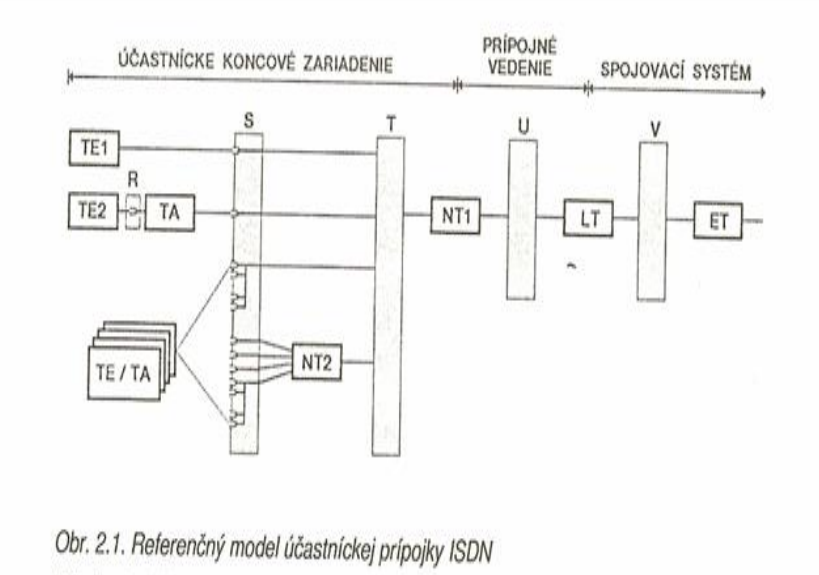
\includegraphics[scale=0.6]{snimky/ISDN-ref.png}
    \end{center}
\end{figure}

\subsection{Rozhraní}
Mezi ISDN sítí a zařízením NT (jednotka ukončení sítě na straně ISDN, na kterou se při základním přístupu připojuje až 8 koncových
zařízení) je použito rozhraní U. Mezi TE (koncové digitální zařízeníbez rozlišení zda slouží pro hlasovou nebo datovou komunikaci) a NT2 (umožňuje připojit několik koncových zařízení současně, což je realizováno sběrnicí, statickým slupovačem nebo i pobočkovou ústřednou.) jsou spojena rozhraním S.

\subsubsection{Struktura rámce S}
Každý rámec obsahuje signalizační informace, pomocné bity, uživatelská data a synchronizaci.
\begin{itemize}
    \item F (Framing Bit) -- bity začátku rámce.
    \item L (Balancing Bit) -- vyvažovací bit pro odstranění stejnosměrné složky.
    \item D (Channel Bit) -- bit D kanálu.
    \item E (Echo Channel Bit) -- bit echo kanálu.
    \item S -- rezervováno pro budoucí využití a je nastaveno na hodnotu 0.
    \item A -- bit použitý pro protokoly aktivace.
    \item B1,B2 -- bity kanálů B1 a B2
\end{itemize}
V kanálu E Slouží k řízení přístupu k D a B kanálům jednotlivým koncovýmzařízením.V případě B kanálu přístup k médiu řídí ústředna.

\subsubsection{Struktura rámce U}

Tvořené dvoudrátovým vedením s plně duplexním provozem. Vedení má maximálně 8km a obsahuje zdroj a opakovač s rozhraním U. Dva druhy kódování:
\begin{itemize}
    \item 4B/3T -- 4 bity do se kódují do 3 ternálních signálů
    \item 2B/1Q -- 2 bity se kódují do jedné značky
\end{itemize}

\subsection{Napájení terminálů}
Napájení terminálu ISDN lze získat v interním napáječi terminálu (charakteristické pro PC), ze síťového napáječe NT fantomním\footnote{Termín \enquote{fantomové napájení} vznikl v 60. letech 20. století po úspěšném pokusu spojit datové a napájecí vedení do jednoho kabelu.} způsobem, ze zdroje jiného terminálu přes přídavný pár vodičů a jednotku NT, z ústředny přes NT a rozhraní S0 fantomním způsobem (použije se při výpadku proudu v místě terminálu).

\clearpage
\section{Asynchronní přepravní způsob -- ATM, buňka ATM, synchronizace, virtuální cesta a virtuální kanál, třídy služeb, ATM vrstvový model, síťové prvky ATM.}

Standard pro síťovou vysokorychlostní architekturu v 80. a 90. letech. Zajišťuje kvalitu služby QoS především pro přenos hlasu a videa. Pracuje s buňkami konstantní délky. ATM je kvalitní technologie, ale pro svou složitost je to technologie drahá, proto je většinou nahrazeno mnohem levnějším Ethernetem. Používá statické multiplexování a směrování po virtuálních kanálech. Umožňuje přenosy dat v řádech Gb/s. Asynchronní není však přenos, ale nepravidelný výskyt buňěk během spojení. ATM tedy definuje rozhraní mezi uživatelem a sítí tzv. UNI a mezi přepínači v síti tzv. NNI.

ATM je vlastně paketovým přenosem dat s určitými odlišnostmi:
\begin{itemize}
    \item Provoz se sestavováním spojení
    \item Přenosová cesta buněk se při sestavování spojení určí přiřazením virtuálního spoje mezi koncovými zařízeními (v koncovém provozu). Tím se připraví potřebné provozní prostředky pro virtuální spojení a přidělí se logické kanály. Při datovém přenosu používají všechny pakety (buňky) stejnou spojovací cestu. Pro vybavení spojení se uvolní obsazené provozní prostředky a logické kanály
\end{itemize}

\subsection{Buňka v ATM}
\begin{figure} [h]
    \centering
    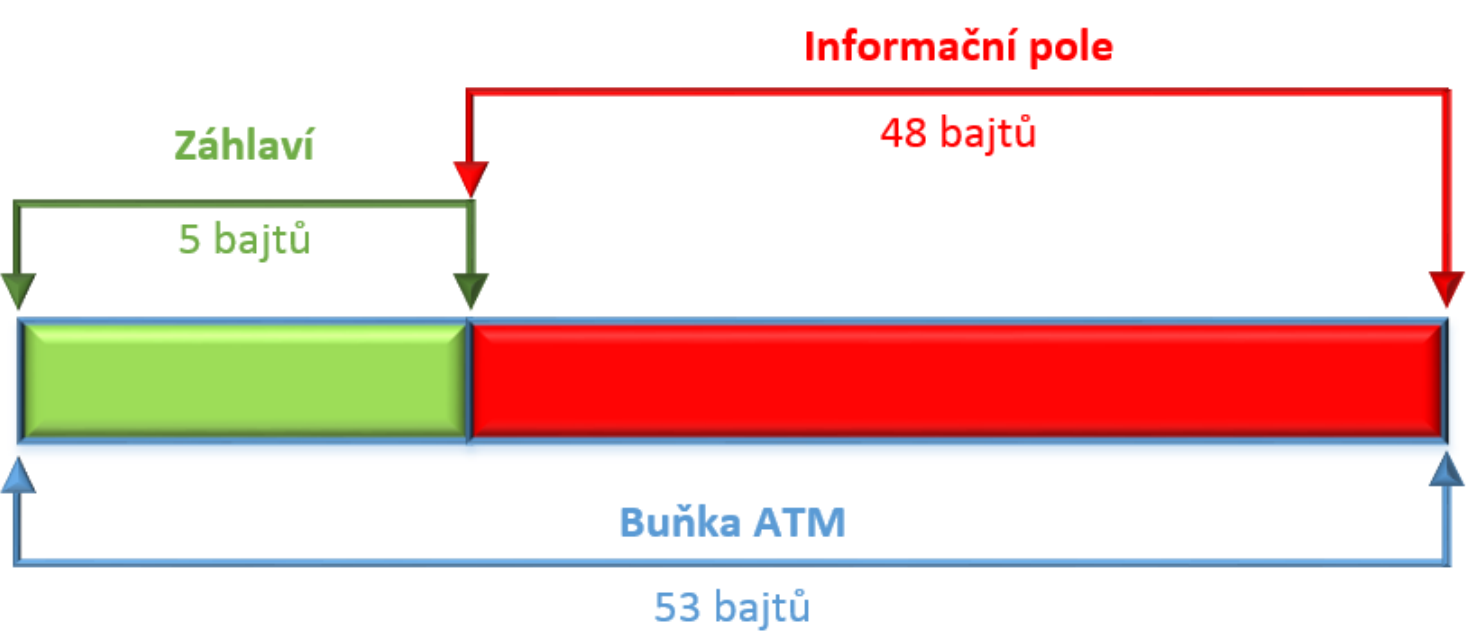
\includegraphics[width=0.5\textwidth]{snimky/ATM bunka.png}
    \label{fig:atm-bunka}
\end{figure}

\subsubsection{Formát hlavičky buňky}
\begin{itemize}
    \item VPI -- Virtual Path Identifier
    \item VCI -- Virtual Circuit Identifier
    \item PT -- Payload Type
    \item CLP -- Cell Loss Priority
    \item HEC -- Header Error Control
\end{itemize}

Rozlišují se dva základní druhy rozhraní:
\begin{itemize}
    \item UNI (User Network Interface) -- rozhraní \enquote{účastník-síť},
    \item NNI (Network Node Interface) -- rozhraní mezi ATM ústřednami.
\end{itemize}

\subsubsection{Synchronizace}
Ke generování jednotlivých buně dochází podle potřeby, zda zdroj má vysílat informace. V opačném případě se přenášejí prázdné buňky. Takto se dosáhne
plynulého toku jednotlivých buněk. Jedná se o asynchronní přenos a to proto, že přenosová bitová rychlost, kterou zdroj vyžaduje je nezávislá na celkové přenosové rychlosti.  Vlastní přenos bitů probíhá synchronně.

\subsection{Virtuální cesty a kanály}
K jedné virtuální cestě VP (Virtual Path) je možno přiřadit několik virtuálních kanálů VC. (Virtual Channel). Takovýmto přiřazením VC jsou propojeny virtuální cesty. V síti ATM je rozlišováno několika prvků, které zajišťují datový přenos:

\begin{itemize}
    \item digitální rozvaděč ATM (ATM Cross-Connect) -- vyhodnocuje identifikátor VPI a VCI
    \item koncentrátor ATM -- vyhodnocuje identifikátory VPI a VCI pro koncentraci provozu
    \item ústředna ATM -- propojuje virtuální spoje v závislosti na VPI a VCI
\end{itemize}

\begin{figure} [h]
    \centering
    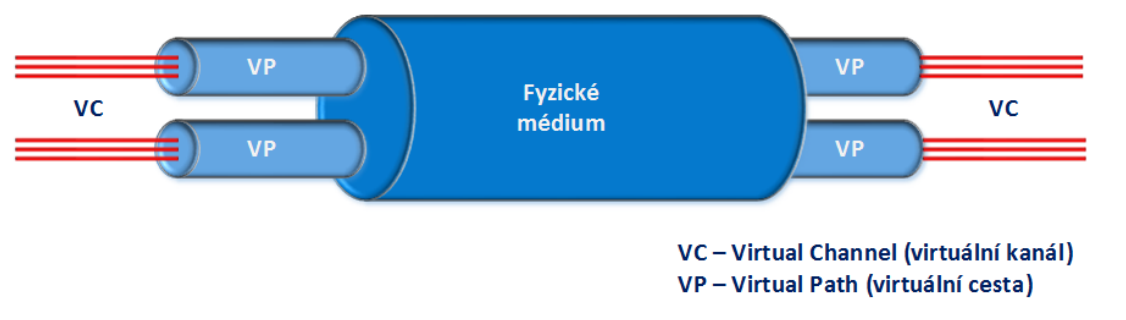
\includegraphics[width=0.8\textwidth]{snimky/VC.png}
    \label{fig:virt-cesty-kanaly}
\end{figure}

\subsection{Třídy služeb}
Pro přenos užitných dat v systémech ATM jsou stanoveny celkem 4 třídy služeb (třídy A až D). Od požadovaných tříd služeb jsou odvozeny různé typy služeb pro přizpůsobení užitných dat při přenosu ATM.

\begin{figure}[h]
    \centering
    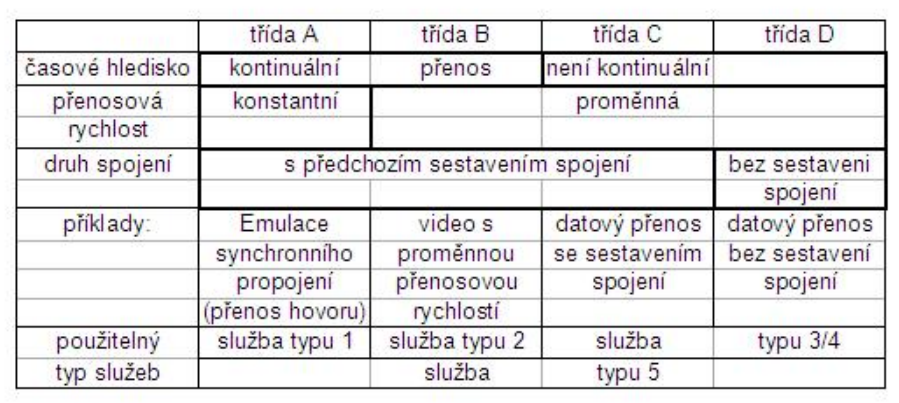
\includegraphics[scale=0.6]{snimky/sluzby.png}
\end{figure}
\newpage

\subsection{Vrstvový model ATM}
\begin{figure} [h]
    \centering
    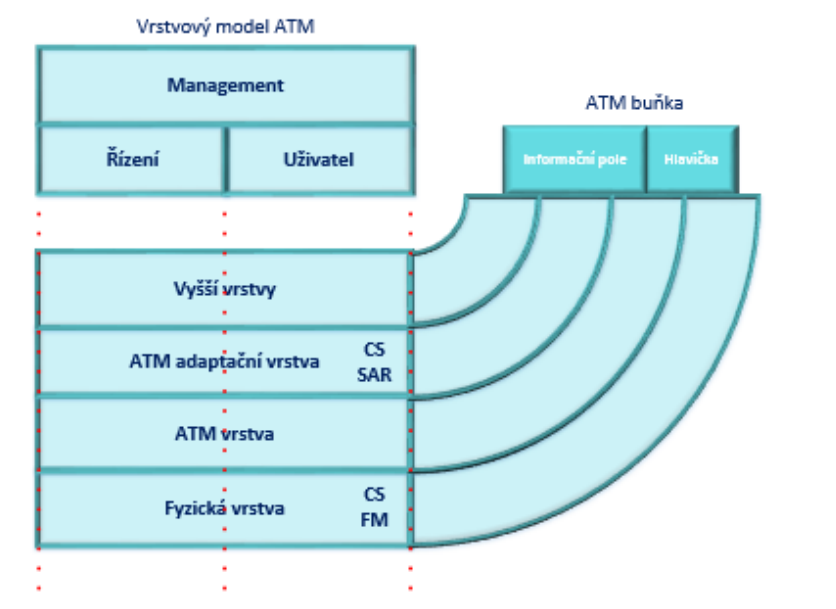
\includegraphics[width=0.5\textwidth]{snimky/ATM model.png}
    \label{fig:vrstvovy-model-atm}
\end{figure}
Vrstvy:
\begin{itemize}
    \item \textbf{Fyzická vrstva} -- rozdělena do dvou částí:
          \begin{itemize}
              \item PMD (Physical Medium Dependent) podvrstva -- synchronizuje vysílánía příjem, určuje fyzické médium včetně typů konektorů a kabeláže.
              \item TC(Transmission Convergence) podvrstva -- má čtyři funkce: vyčleňování buněk, kontrolu záhlaví pomocí (HEC) sekvence, přizpůsobení přenosu rámců.
          \end{itemize}
    \item \textbf{ATM vrstva} -- Poskytuje následující funkce -- generic Flow Control (GFC)( řešení vícenásobného přístupu na UNI),přiřazuje hodnoty VPI a VCI každé buňce a poskytuje překlady VCI/VPI, multiplex buněk.
    \item \textbf{Adaptační vrstva ATM}
          \begin{itemize}
              \item AAL1 -- poskytuje spojově orientovanou službu a provádí emulaci okruhů pro aplikace, jako jsou například hlasové nebo videokonference. Požaduje synchronizaci zdroje a vysílače. Tato vrstva je závislá na typu média, které musí podporovat taktování.
              \item AAL2 -- poskytuje efektivní přidělování šířky pásma, obsahuje krátké a variabilní pakety
              \item AAL3/4 -- poskytuje jak spojově orientovanou službu, tak i spojově neorientovanou službu.
              \item AAL5 -- primární vrstvou pro data AAL a definuje jak spojově orientovanou službu, tak i spojově neorientovanou.
          \end{itemize}
\end{itemize}


\clearpage
\section{Digitální účastnická přípojka xDSL, HDSL, ADSL, spojení, referenční model, modulace, rušivé vlivy, přeslechy.}
\subsection{xDSL -- Digital Subscriber Line}

Využívá stávajícího vedení telefonní sítě k uživateli. Jednotlivé typy DSL se liší použitým frekvenčním pásmem, přenosovou
rychlostí a možným dosahem. Obecně platí, že čím horším je vedení od ústředny k uživateli (kvalita
rozvodu a délka), tím menší je přenosová rychlost. Nejčastějším typem DSL je stále ještě ADSL, postupně je však nahrazováno
sofistikovanějšími a rychlejšími technologiemi. ADSL, VDSL, HDSL a další jsou označované pod souhrnným názvem xDSL. Jsou rozlišovány dvě základní verze xDSL technologie:
\begin{itemize}
    \item Symetrická -- symetrická řešení poskytují jak v dopředném, tak i v opačném směru synchronní přenos dat.
    \item Asymetrická -- ADSL
\end{itemize}

\subsubsection{Metody zabezpečení proti chybám v DSL}
\begin{itemize}
    \item Detekce chyb pomocí cyklického kódu CRC
    \item Dopředná chybová korekce FEC -- Spolu s prokládáním poskytuje FEC ochranu hlavně proti shlukům chyb. Skramblování neslouží k opravě chyb, ale rozrušuje dlouhé posloupnosti jedniček a nul a tak zabezpečí lepší synchronizaci na přijímací straně.
    \item Interleaving -- ochrana zabezpečení dat při přenosu v prostředí, zarušené především impulsním šumem. Zvyšuje odolnost přenosu, ale vnáší do přenosu větší zpoždění.
\end{itemize}

\subsection{ADSL}
Zajišťuje datový přenos vyššími rychlostmi po symetrickém vedení. Na obou koncích vedení instalovány transceivery, a to s modulacemi DMT, QAM či CAP. Používá existující dvoudrátové vedení pro vysokorychlostní přenos dat se zachováním služby POTS, přenos je full duplex.
\subsubsection{Referenční model}
\begin{figure} [h]
    \centering
    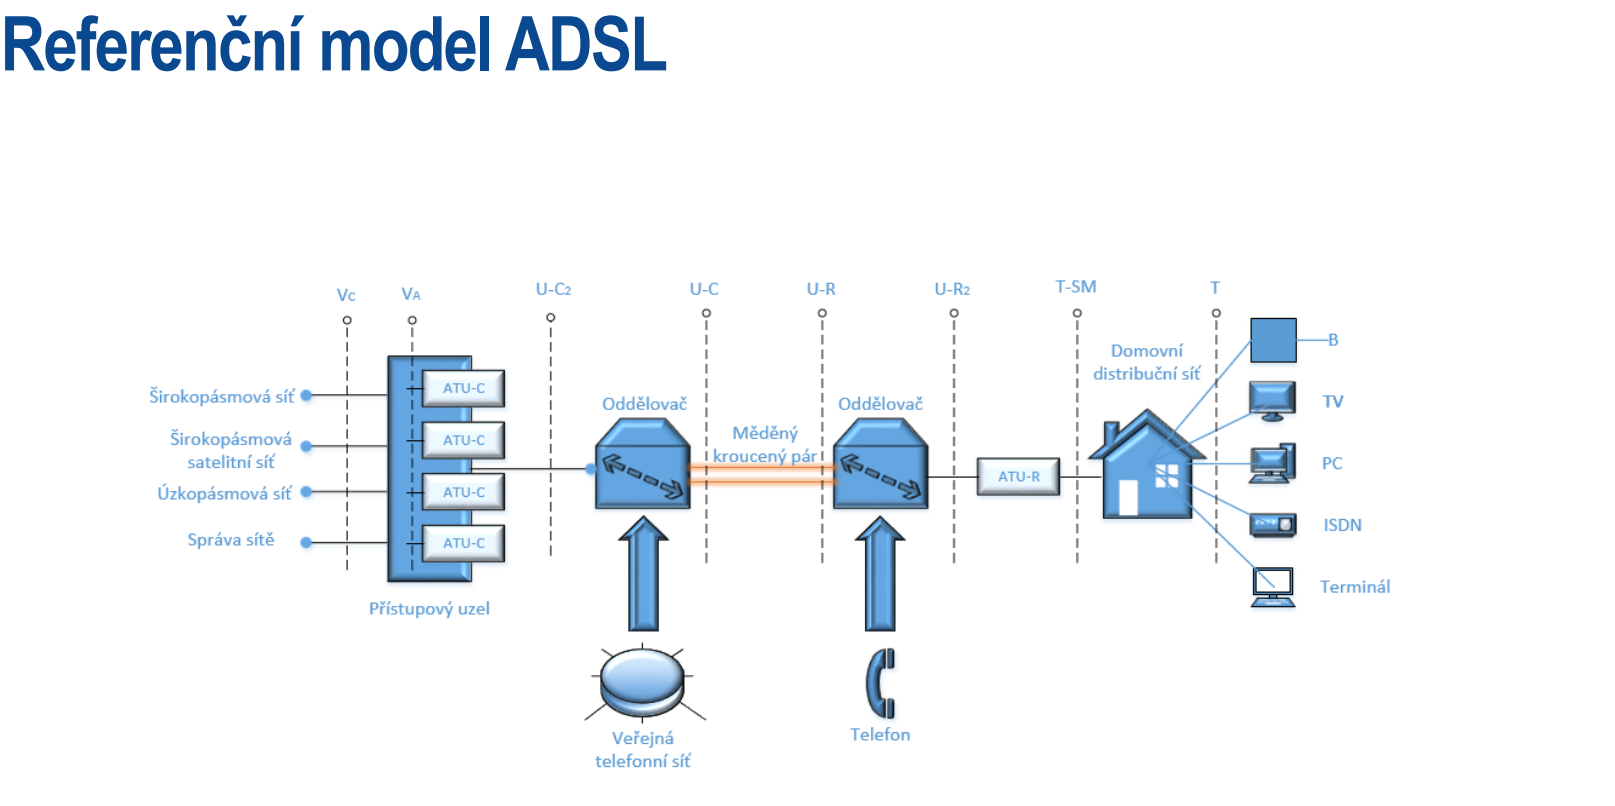
\includegraphics[scale=0.85]{snimky/ADSL model.png}
\end{figure}
\newpage
\subsubsection{Spojení (asi myslel zapojení...)}
\begin{figure} [h]
    \centering
    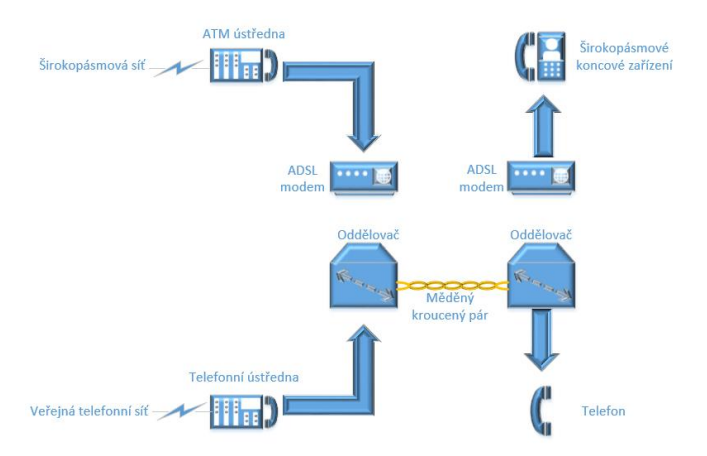
\includegraphics[scale=0.8]{snimky/zapoj.png}
\end{figure}

Hlavní komponenty sítě:
\begin{itemize}
    \item DSLAM (DSL Access Multiplexer) -- slučuje hlasový provoz a DSL provoz na jednu telefonní linku (dvoudrát),pracuje na L2 vrstvě jako switch, funkce tzv. přístupového koncentrátoru, k jednomu DLSAMu lze připojit až několik tisíc uživatelů, záleží na počtu portů dané karty.
    \item ADSL modem -- modem pro přípojku, k PC se připojuje přes Ethernet, popř. USB.
\end{itemize}

\subsubsection{Modulace}
Využíva se kvadraturní amplitudová modulace QAM, amplitudová fázová modulace bez nosné CAP, diskrétní vícetónová modulace DMT.
\begin{itemize}
    \item QAM -- používaná ve velké řadě aplikací (např. modemy v základním pásmu, mikrovlnné radiové systémy aj.). Modulace se provádí pomocí digitálního kvadraturního (ortogonálního) modulátoru se sinusovou a kosinusovou směšovací funkcí. Díky této ortogonalitaě (nosných signálů) se umožní následná detekce dat v přijímači.
    \item CAP -- podobná QAM. Používá stejné dvourozměrné přenosové schéma a má stejný typ výkonového spektra. Modulace se provádí pomocí digitálních transverzálních pásmových filtrů. Impulsní odezva těchto filtrů má stejnou amplitudovou charakteristiku, ale fázová charakteristika se navzájem liší o 90°.
    \item \textbf{DMT} -- jeví se v systémech ADSL jako velmi perspektivní a výrobci podporovaná. Modulace s více nosnými MCM. Je založena na diskrétní Fourierově transformaci, resp. na rychlé Fourierově transformaci FFT (Fast Fourier Transform). Velkou výhodou této metody modulace je plně digitální realizace a poměrně nízká složitost. Pomocí DMT lze efektivněji řešit negativní vlivy nedokonalé přenosové cesty a také rušící vliv okolí na užitečný signál při přenosu symetrickým párem v metalické přístupové síti
\end{itemize}
\newpage

\subsubsection{Rušivé vlivy}
\begin{figure} [h]
    \centering
    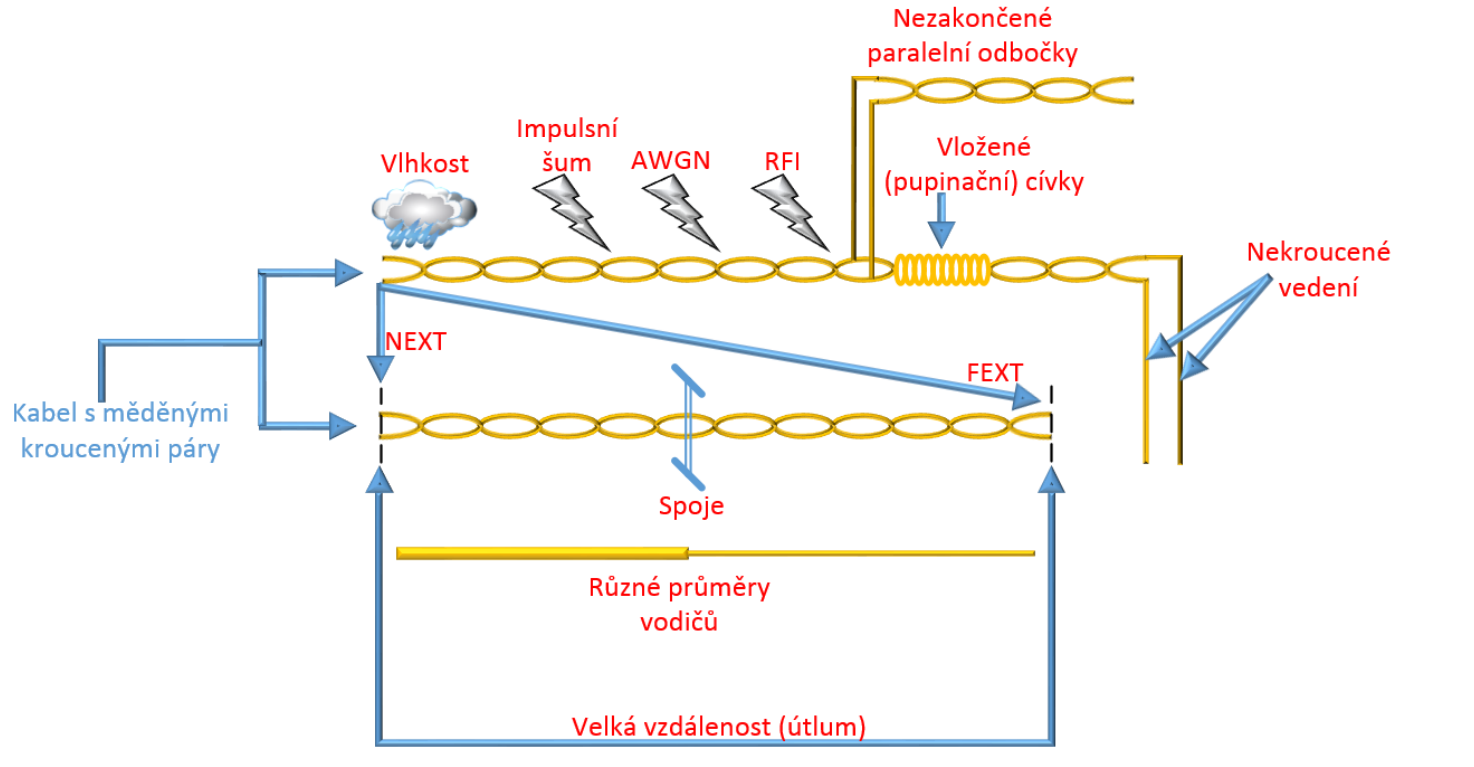
\includegraphics[width=0.8\textwidth]{snimky/ADSL ruch.png}
    \label{fig:adsl-ruch}
\end{figure}
\begin{itemize}
    \item Vnější rušivé vlivy
    \item Impulsní rušení -- impulsive noise
    \item Vf rušení -- RFI (Radio Frequency Interference)
    \item Vnitřní rušivé vlivy
    \item NEXT (Near And cross talk)
    \item FEXT (Far End cross Talk)
    \item AWGN (Additive White Gausian Noise)
\end{itemize}

\subsubsection{Přeslechy}
NEXT, FEXT
Aditivní bílý šum (Tepelný šum, Výstřelový šum, Kvantizační šum, Zbytkový odrazový šum)

\subsection{HDSL}
V případě varianty T1 používá 2 páry telefonního vedení, každý o rychlosti 784 kb/s. V případě E1 varianty 1168 kb/s na každý pár. Používají se modulace 2B1Q a CAP. Jednotlivá maximální délka vedení mezi HDLS je 3,7 km v případě modulace 2B1Q nebo 4,2 km

\clearpage
\section{IPv6, návaznost na IPv4, kvalita služeb QoS, referenční model OSI versus síťová architektura TCP/IP.}

\subsection{IPv6}
Nahrazuje dosluhující protokol verze 4. Masivní rozšíření adresního prostoru. Zdokonalení vysokorychlostního přenášení dat. Pro uživatele není nutná žádná specifická příprava. Nutná podpora ze strany sítě. IPv6 nahrazuje formát IP datagramů. Velikost hlavičky je 40 bajtů a Payload 64 KB. Pro adresaci v IPv6 se používá adresování založené na CIDR (Classless Inter-Domain Routing).

Typy adres:
\begin{itemize}
    \item Unicast -- unikátní -- adresace rozhraní
    \item Anycast -- speciální typ adresy, kterým je definováno více rozhraní, ale provoz je směrován pouze jednomu, většinou nejbližšímu rozhraní z logického pohledu
    \item Multicast -- vícesměrová adresa
\end{itemize}

\subsubsection{Návaznost IPv6 na IPv4 protokol}
Základním rozdílem protokolu IPv4 a IPv6 je v rozsahu použitelných adres v síti pro jednotlivá rozhraní, zařízení. Technické funkce fungování sítí zůstávají stejné a obě verze jsou provozovány současně. IPv4 -- adresní rozsah 32 bitový, IPv6 128 bitový.

\subsection{Quality of Services}
K základním metrikám (požadavkům) patří \textbf{komunikační zpoždění} (paketové, rámcove, zpoždění kódováním), \textbf{jitter} (nežádoucí odchylku periodického signálu a vyjadřuje nestabilitu zdroje), \textbf{šířka pásma, ztráta rámců a paketů} (důvodu rušení přenosové linky, nebo zahlcením jednotlivých kapacit prvků sítě, které mají omezenou schopnost odbavovat provoz a po naplnění jednotlivých vstupních front začnou provoz zahazovat), míra pravděpodobnosti blokování (vyjádřeno modely Erlang), \textbf{kvantovací šum} (vázán na zdrojové kódování a jeho vzorkovací
a kvantovací procesy), \textbf{objektivní a subjektivní testování} (měří a vyjadřuje se v jednotkách MOS (Mean of Services) vnímání kvality služby uživatelem takovéto služby).

\subsubsection{Služby}
\begin{itemize}
    \item Služby \enquote{Best Effort} -- jedná se o typ služby s maximálním úsilím o přenos v síti, bez specielního nastavení QoS v takovéto síti. Nejlépe je charakterizováno pomocí plánování front metodou FIFO (First In First Out).
    \item Služby integrované \enquote{IntServ} -- takovýto model QoS rezervuje požadavky síťového provozu po celou dobu trvání přenosu. Aplikace si sami určují nároky na přenos (oznamují je síťovým prostředkům, jako jsou směrovače). Je zde využito například protokolu RSVP (Resource Reservation Protocol).
    \item Služby diferencované \enquote{DiffServ} -- v tomto modelu poskytování QoS dochází již ke klasifikaci jednotlivých přenosů. Je zde použito metod QoS jako je například metoda WFQ (Weighted Fair Queueing), WRED (Weighted Random Early Detection). Požadavky na QoS neurčují aplikace, ale zařízení v síti.
\end{itemize}

\subsubsection{QoS IPv6}
V IPv4 je obvykle provozována služba \enquote{Best Effort} tedy nejlepší snaha o přenos informační jednotky. Fragmentace paketů je v IPv4 hlavním zdrojem zpoždění paketů nebo jejich vysoké latence. IPv6 používá sofistikovanější přístup k zpracování dat. IPv6 má dvě pole týkající se QoS, a to 20 bitové pole \enquote{Flow Label} a 8 bitové pole \enquote{Traffic Class}.


\subsection{Referenční model OSI}
Sedm vrstev k zajištění protokolové komunikaci mezi zařízeními. Základní myšlenkou je, že každá z vrstev komunikuje pouze s vrstvou
vlastní horizontálně pomocí jednotek PDU (Packet Data Unit). Mezi jednotlivými vrstvami jsou stanovená pevně definovaná rozhraní
komunikující ve vertikálním směru provádějící servisní operace mezi vrstvami nazývané SDU (Service Data Unit). Každá z nižších vrstev přidá své PDI (Protocol Control Information) k datům, která převzala od vrstvy vyšší.
\begin{figure} [h]
    \centering
    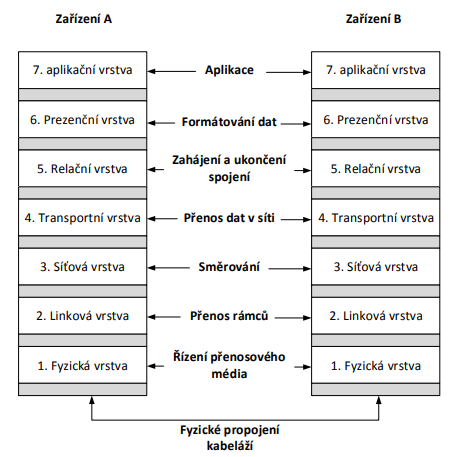
\includegraphics[width=0.5\textwidth]{snimky/osi.png}
    \label{fig:osi}
\end{figure}

\begin{itemize}
    \item fyzická vrstva -- zajišťuje spojení mezi zařízeními na fyzické úrovni, poskytuje služby zpracování signálu. Definuje základní zpracování a přenos informací v signálové části a přizpůsobení se fyzickému médiu. Základní jednotka \textit{bit}.
    \item linková vrstva -- zajišťuje přenos a zpracování \textbf{rámců} v rámci segmentu. Pro vyšší vrstvu zajišťuje bezporuchovou službu a spojení mezi dvěma síťovými prvky.
    \item síťová vrstva -- zajišťuje směrování \textbf{paketů} a její úlohou je najít nejvhodnější cestu v síti pro přenos informace.
    \item transportní vrstva -- zajišťuje řízení komunikace mezi odesílatelem a příjemcem a poskytuje přenos a zpracování jednotek \textbf{TCP segmentů} a \textbf{UDP datagramů}.
    \item relační vrstva -- zajišťuje navázání, udržování a ukončení relací mezi jednotlivými účastníky spojení. Při navazování spojení si vyžádá od transportní vrstvy vytvoření relace. \textbf{Data}
    \item prezenční vrstva -- zajišťuje kódování, překlad, konverzi, šifrování a kompresi přenášených informací. Je zde zaveden společný jazyk pro konverzi údajů ASN.1. (Abstract Syntax Notation One). Dále se sem řadí protokoly TLS, starší SSL. \textbf{Data}
    \item aplikační vrstva -- provádí správu aplikačních systémů a programů. Mezi protokoly řadící se do této vrstvy patří HTTP, FTP, POP3, SNMP, AIM, DHCP a jiné. \textbf{Data}
\end{itemize}

\subsection{Porovnání ISO/OSI a TCP/IP}
\begin{figure} [h]
    \centering
    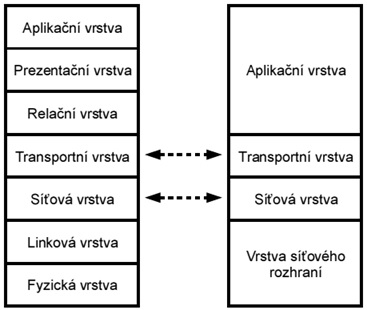
\includegraphics[scale=0.85]{snimky/Vrstvy2.jpg}
\end{figure}

\clearpage
\section{Pasivní optické sítě (topologie sítě a způsob komunikace sestupný/vzestupný směr).}
Pasivní optické sítě (PON) se skládají z:
\begin{itemize}
    \item OLT -- je řídící jednotka, která řídí celou funkcionalitu PON pro obousměrnou komunikaci.
    \item ONU -- optická síťová jednotka realizující převod z optického signálu na elektrický signál nebo naopak.
    \item Splitter -- rozděluje optický signál na více signálů
\end{itemize}
\begin{figure} [h]
    \centering
    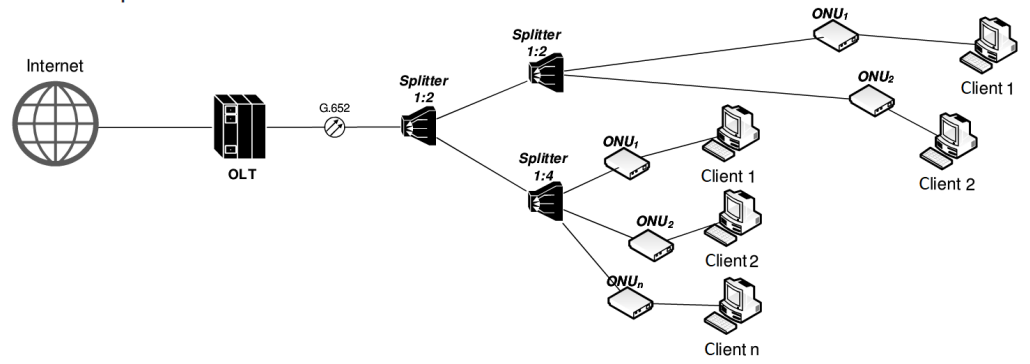
\includegraphics[width=\textwidth]{snimky/PONTopologie.png}
    \label{fig:pon}
\end{figure}

Komunikace probíhá v sestupném směru jako broadcast, kdy splitter rozesílá data na všechny jednotky ONU v poměru 1:N. ONU jednotka zkontroluje identifikátor (nejspíše ONU-ID) přijatého rámce a pokud se identifikátor shoduje s přiřazeným identifikátorem tak data příjme. V opačném případě data zahodí. Tyto data se poté přenáší k cílové OLT kdy jsou spojována do jednoho signálu. Viz obrázek.

\begin{figure} [h]
    \centering
    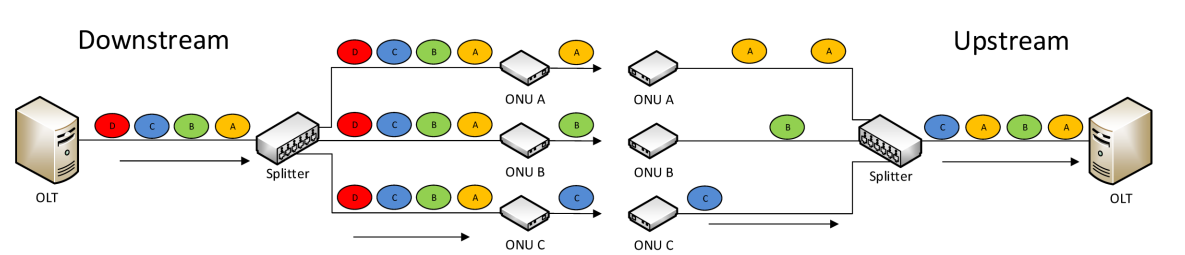
\includegraphics[width=\textwidth]{snimky/upDownPON.png}
\end{figure}

Pro realizaci obou směrů na jednom vlákně lze využít např. dělení podle času, nebo vlnové délky.
\clearpage
\section{Vývoj pasivních optických sítí a jejich rozdíly z pohledu fyzické a přenosové vrstvy.}

\subsection{ATM PON (APON) a BPON}
Rychlost v symetrické variantě 155,52\,MB/s a v asymetrické 622,8/155,52\,MB/s. BPON vylo pouze rozšíření a zvyšovala symetrickou rychlost na 622.8\,MB/s a přidávala nové funkce jako dynamickou distribuci pásma, vlnový multiplex (WDM).

\subsection{GPON}
GPON je nejpoužívanější v ČR. Využívá linkový kód NRZ (Non-return-to-zero) a podporuje plně ethernetové rámce se zapouzdřením do rámců GEM (Gigabit Passive Optical Network Encapsulation Mode) viz obrázek. Přenosové rychlosti závisí na použité variantě (symetrická/asymetrická).

\begin{figure} [h]
    \centering
    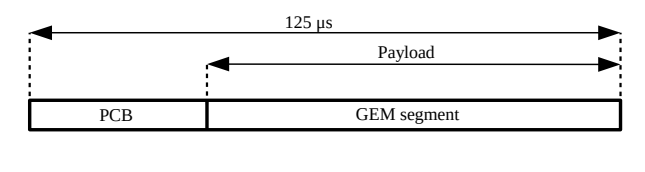
\includegraphics[width=\textwidth]{snimky/gemFrame.png}
\end{figure}

\subsection{EPON}
Odvozen od standardního Ethernet protokolu. Využívá linkový kód 8B/10B, tj. ke každému bloku 8 bitů jsou přidány 2 paritní bity. Pro přenos se využívá Ethernet rámců viz obrázek. Předchází kolizi paketů v síti pomocí MPCP (MultiPoint Control Protocol). Funguje na principu detekce ONU a ustanovení provozních parametrů, kdy na konci je mu přiděleno LLID.

\begin{figure} [h]
    \centering
    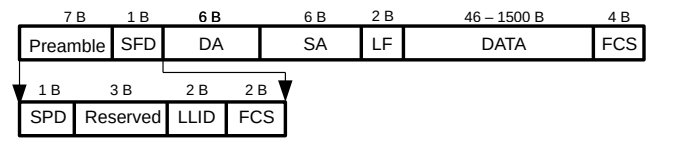
\includegraphics[width=0.8\textwidth]{snimky/EPONframe.png}
\end{figure}

\begin{itemize}
    \item SPD obsahuje informace o hodinovém signálu
    \item Reserved jsou tři byty pro budoucí účely
    \item LLID je identifikátor ONU
    \item FCS -- informace o detekci chyb
\end{itemize}

\clearpage

\begin{table}[ht]
    \centering
    \caption{GPON vs EPON (nevím jestli je ta přenosová vrstva správně)}
    \begin{tabular}{|l|l|l|}
        \hline
                                     & GPON           & EPON           \\\hline\hline
        \textbf{Fyzická vrstva}      &                &                \\\hline\hline
        Downstream [Gb/s]            & 1,244/2,488    & 1,25           \\\hline
        Upstream [Gb/s]              & 1,244/2,488    & 1,25           \\\hline
        Downstream vlnová délka [nm] & 1480\,--\,1500 & 1480\,--\,1500 \\\hline
        Upstream vlnová délka [nm]   & 1260\,--\,1360 & 1260\,--\,1360 \\\hline\hline
        \textbf{Přenosová vrstva}    &                &                \\\hline\hline
        Protokol                     & GEM            & Ethernet       \\\hline
        Linkové kodovaní             & NRZ            & 8B/10B         \\\hline
        Zabezpečení                  & downstream     & obousměrně     \\\hline
        Max dělící poměr             & 1:64           & 1:32           \\\hline
        Max dosah sítě [km]          & 20             & 20             \\\hline
    \end{tabular}
\end{table}

\subsection{XG-PON a XG(S)-PON}

XG-PON vylepšuje GPON, hlavně v nově použitém protokulu XGEM.

XGS-PON je pouze rozšíření XG-PON, kdy hlaví změnou je nově navržená TC (Transmission Convergence) vrstva, která je odvozena od standardu NG-PON2.

\subsection{10G-EPON}

Navazují standard na EPON s cílem možnosti provozovat 10G-EPON v souběhu s EPON na stejné optické distribuční síti.

\subsection{NG-PON2}
Poslední kompletně standardizovaný standard pro PON.

NG-PON2 umožnuje rychlost 40\,Gb/s s možností škálování až k hranici 80\,Gb/s. Využívá TWDM. TWDM pro vzestupný směr využívá tří typů pásem 1524-1544 (široké), 1528-1540 (zúžené) a 1532-1540 (úzké).

\begin{table}[ht]
    \centering
    \caption{XG(S)-PON vs 10G-EPON vs NG-PON2}
    \begin{tabular}{|l|l|l|l|}
        \hline
                                     & XG(S)-PON      & 10G-EPON       & NG-PON2                            \\\hline\hline
        \textbf{Fyzická vrstva}      &                &                &                                    \\\hline\hline
        Downstream [Gb/s]            & 9,9533         & 10,3125        & 40                                 \\\hline
        Upstream [Gb/s]              & 2,4883(9,9533) & 10,3125        & 10(asymetrický)/40(symetrický)     \\\hline
        Downstream vlnová délka [nm] & 1575\,--\,1580 & 1575\,--\,1580 & 1596\,--\,1603                     \\\hline
        Upstream vlnová délka [nm]   & 1260\,--\,1280 & 1260\,--\,1280 & 1524/1528/1533\,--\,1544/1540/1540 \\\hline\hline
        \textbf{Přenosová vrstva}    &                &                &                                    \\\hline\hline
        Protokol                     & XGEM           & Ethernet       & XGEM                               \\\hline
        Linkové kodovaní             & NRZ            & 64B/66B        & NRZ                                \\\hline
        Zabezpečení                  & obousměrně     & obousměrně     & obousměrně                         \\\hline
        Max dělící poměr             & 1:64           & 1:32           & 1:64                               \\\hline
        Max dosah sítě [km]          & 20             & 20             & 20                                 \\\hline
    \end{tabular}
\end{table}

\subsection{Super-PON}
\begin{itemize}
    \item Zvyšuje počet připojených ONU k jediné OLT z 64 na 1024
    \item Dochází ke snížení počtu CO, protože dosah sítě je zvýšen z 20 na 50 km
    \item Nasazení od 10 Gbit/s po 25 Gbit/s –> využití pro sítě 5G
\end{itemize}

\subsection{Higher Speed PON (HSP)}
Parametry:
\begin{itemize}
    \item Přenosová rychlost – sestupný směr: 49,77 Gbit/s
    \item Přenosová rychlost – vzestupný směr: 49,77/24,88/12,44 Gbit/s
    \item Samo opravný kód: LDPC (low-density parity check)
    \item Linkový kód: NRZ
    \item Maximální vzdálenost přenosu: 20–40km
    \item Použitá vlnová délka 1340–1344nm
\end{itemize}

\clearpage
\section{Aktivační proces koncové jednotky v síti GPON.}
V současné době je GPON jedním z nejslibnějších řešení pro přístupové sítě (z pohledu ceny). GPON byl první standard, který podporoval přenos/zapouzdření ATM buněk i Ethernet rámců.

Aktivační proces:
\begin{figure} [h]
    \centering
    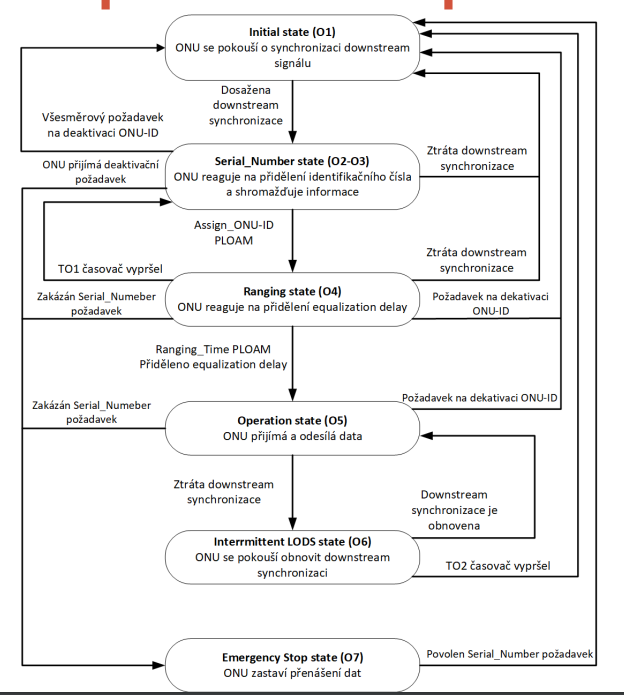
\includegraphics[width=0.63\textwidth]{snimky/proces.png}
    \label{fig:gpon-proces}
\end{figure}

Jednotka ONU komunikuje s OLT pomocí PLOAM zpráv, kdy typy zpráv a průběh komunikace je vidět níže.

\begin{figure} [h]
    \centering
    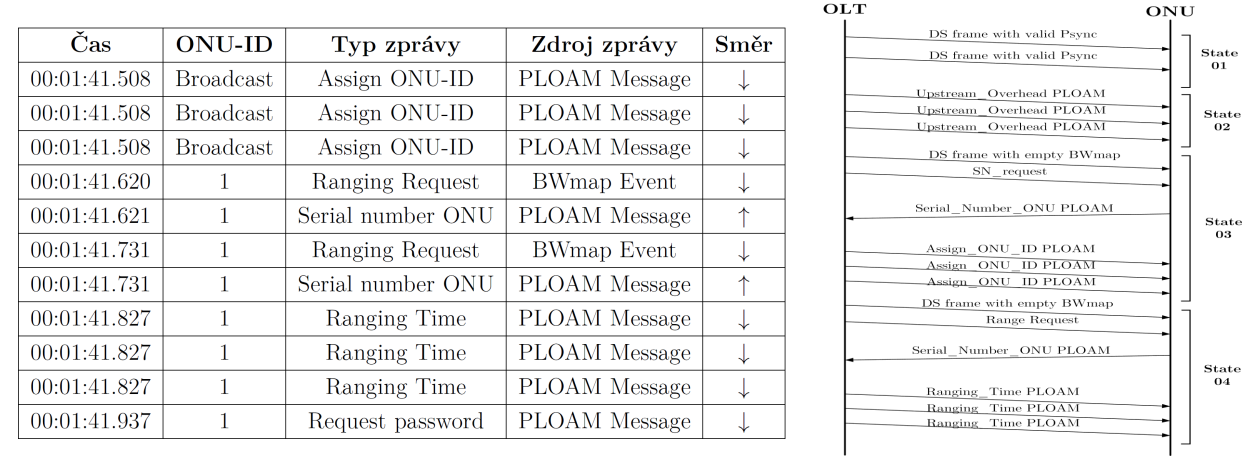
\includegraphics[width=0.9\textwidth]{snimky/aktivaceONU.png}
\end{figure}


\clearpage
\section{Využití celočíselného programování v současných sítích, síť jako graf, rozdělení zátěže z pohledu ceny přenosu.}
\textbf{Lineární programování} je obor matematiky, stejně jako matematika sama. \textbf{Lineární program} je maximalizace nebo minimalizace lineární funkce podléhající lineárním omezením (např. Lineární rovnice nebo lineární nerovnosti). Optimalizační problém s funkcí, která má být maximalizována nebo minimalizována, se nazývá \textbf{matematický program}. Pokud jsou proměnné v matematickém programu omezeny na nezáporná celá čísla, matematický program se nazývá \textbf{celočíselný program}.

\textbf{Realizovatelným/možným řešením} je řešení lineárního programu, které splňuje všechny omezení. Sada všech možných řešení se nazývá prostor pro řešení. Jestli že má lineární program realizovatelné řešení tak říkáme že je proveditelné jinak je neuskutečnitelné.

\subsection{Maximalizace toku}
Problém maximalizace toku hledá toky provozu, které maximalizují objem přenosu ze zdrojového uzlu do cílového, s omezením že není překročena kapacita spoje.

\begin{figure} [h]
    \centering
    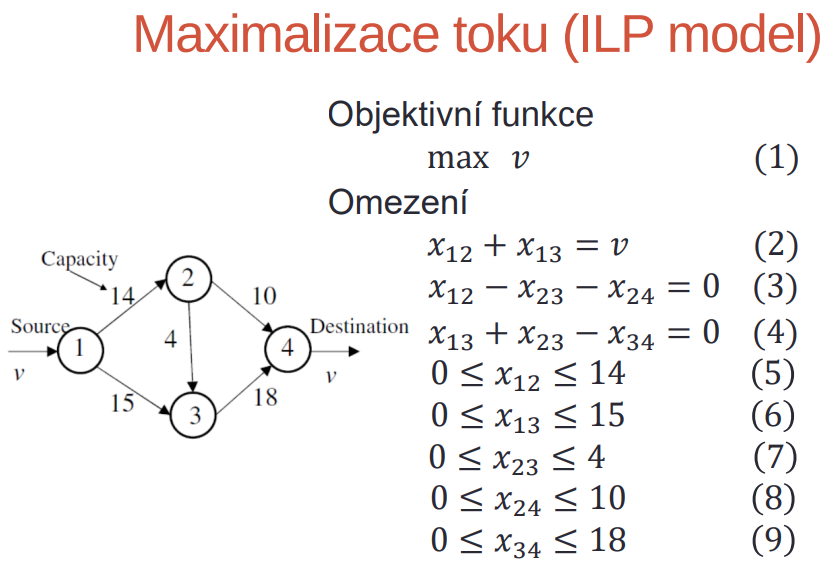
\includegraphics[width=0.8\textwidth]{snimky/ilpModel.png}
\end{figure}

Max v představuje objektivní funkci, která maximalizuje objem provozu od uzlu 1 do uzlu 4. Rovnice 2 -- 9 jsou omezení funkce, kdy rovnice 2 -- 4 ukazují zachování průtoku.

Rovnice 2 ($x_{12} + x_{13} = v$) je omezení udržování toků v uzlu zdroje. Odchozí objem provozu z uzlu 1 je roven $v$.

Rovnice 3 ($x_{12} - x_{23} - x_{24} = 0$) je omezení k udržení toků v uzlu 2. Příchozí objem do uzlu 2 je roven odchozímu provozu z uzlu 2.

Rovnice 4 ($x_{13} + x_{23} - x_{34} = 0$) je omezení k udržení toků v uzlu 3. Příchozí objem do uzlu 3 se rovná odchozímu objemu provozu z uzlu 3.

V případě úlohy na obrázku bude $v = 28$, kdy se bude skládat ze tří cest. První cesta ($1\xrightarrow{}2\xrightarrow{}4$) má maximální tok 10, druhá cesta ($1\xrightarrow{}2\xrightarrow{}3\xrightarrow{}4$) má maximální tok 4 a třetí cesta ($1\xrightarrow{}3\xrightarrow{}4$) má maximální tok 14.

\subsection{Minimální cena toku}

Problematika minimální ceny toku se snaží najít toky, jejich cena je minimalizována tak, aby splňovala že objem provozu nepřekračuje kapacitu spoje (maximalizace toku).

\begin{figure} [h]
    \centering
    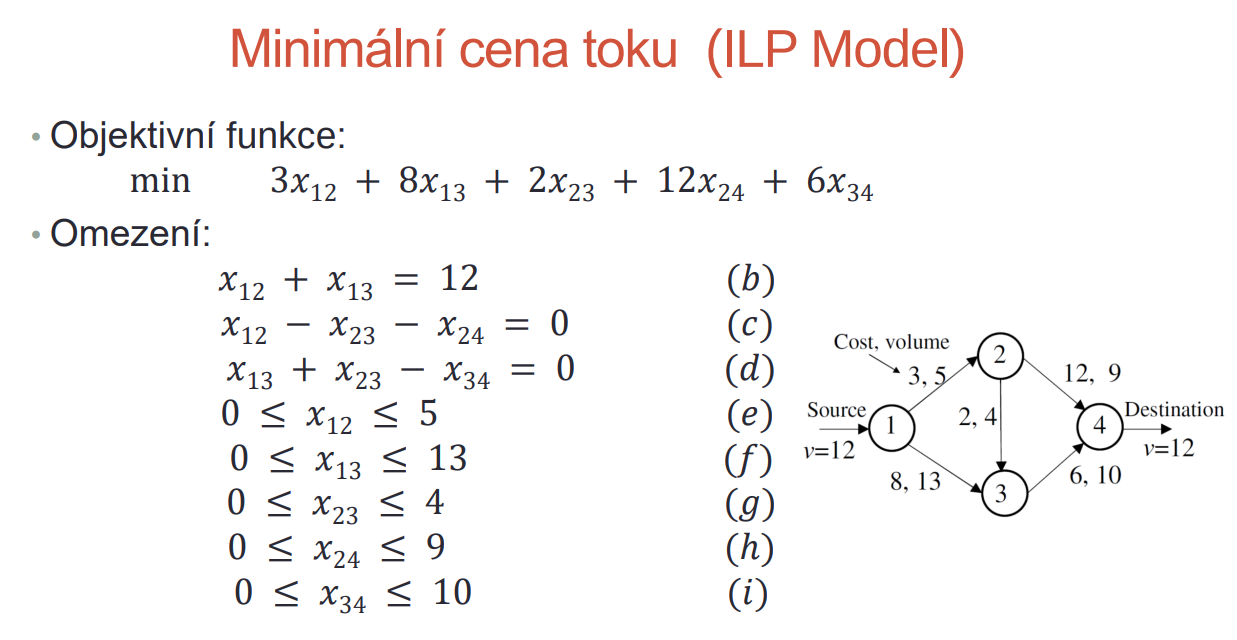
\includegraphics[width=0.8\textwidth]{snimky/MinCena.png}
\end{figure}

Na obrázku dvojice čísel u hran představuje cenu, kapacitu. Definice rovnic na obrázku jsou stejné jako v případě maximálního toku. Jen zde se hledá výsledná minimální cena.

V případě úlohy na obrázku bude $v = 12$ a celková cena je 161, kdy se bude skládat ze tří cest. První cesta ($1\xrightarrow{}2\xrightarrow{}4$) má maximální tok 2, druhá cesta ($1\xrightarrow{}2\xrightarrow{}3\xrightarrow{}4$) má maximální tok 3 a třetí cesta ($1\xrightarrow{}3\xrightarrow{}4$) má maximální tok 7.



\clearpage
\section{IP přenos sítí wavelength division multiplexing (WDM), CWDM, DWDM, TDM versus WDM, problematika přiřazování vlnových délek (RWA).}

\subsection{Vlnový multiplex WDM}

Přenos více signálů jedním optickým vláknem v rozdílných vlnových délkách. Je základem pro všechny rozšiřující vlnové multiplexy.

\subsubsection{IP přes WDM}

Slouží k přenosu IP protokolu v optické síti s podporou WDM. IP jako technologie síťové vrstvy spoléhá na vrstvu datového spojení poskytující rámcování, detekci chyb, obnovení chyb (opakování požadavku při chybě). Motivace pro IP/WDM může být, že za využití stávající infrastruktury, lze pomocí WDM zvýšit šířku pásma vláken. Většina přenosů mezi sítěmi využívá IP a zároveň většina uživatelských aplikací podporuje IP.

\subsection{Vlnový multiplex CWDM }
Označovaný jako \enquote{hrubý}, umožňuje v jediném optickém vlákně přenášet najednou až 18 nezávislých optických signálů s různou vlnovou délkou. Každý přenášený optický signál o dané vlnové délce může nést odlišnou informaci s různou přenosovou rychlostí.
Mezi výhody CWDM technologie patří:
\begin{itemize}
    \item nižší pořizovací cena oproti DWDM,
    \item snadná realizace na stávajících optických trasách,
    \item nižší energetické a prostorové nároky v porovnání s DWDM,
    \item jednoduchý management,
    \item velká nabídka vysílačů,
    \item tolerance střední vlnové délky kanálu 6-7 nm.
\end{itemize}

\subsection{Vlnový multiplex DWDM}
Označovaný jako \enquote{hustý}, patří mezi nejdokonalejší technologie. Umožňuje přenášet v jednom optickém vlákně desítky kanálů. Kanály jsou optickým vláknem přenášeny paralelně a nezávisle na sobě, co několikanásobně zvyšuje přenosovou kapacitu optického spoje. Technologie využívá především laserů DFB (Distributed FeedBack) laser s extrémně úzkou spektrální čarou, dále EDFA (Erbium Doped Fiber Amplifier) zesilovače a vysoce selektivní
spektrální filtry. Tato zařízení jsou velice citlivá na kmitočtovou a teplotní stabilitu. To je jedním z důvodů, proč je tato technologie velmi nákladná
Mezi výhody DWDM patří:
\begin{itemize}
    \item umožnují přenosovou rychlost 2,5 až 10 Gbit/s v jednom optickém kanále,
    \item na jednom optickém vlákně dokáže přenést více než 96 datových kanálů,
    \item velký dosah do 100 km bez nutnosti zesílení signálu,
    \item snadná rozšiřitelnost o další datové kanály.
\end{itemize}

\subsection{TDM vs. WDM}
Díky neustálému požadavku na šířku pásma při výstavbě infrastruktury a provozování služeb je relativně drahé položit nová vlákna a dále je
spravovat. Proto jsou nezbytné techniky vícenásobného využití vlákna.
\begin{figure} [h]
    \centering
    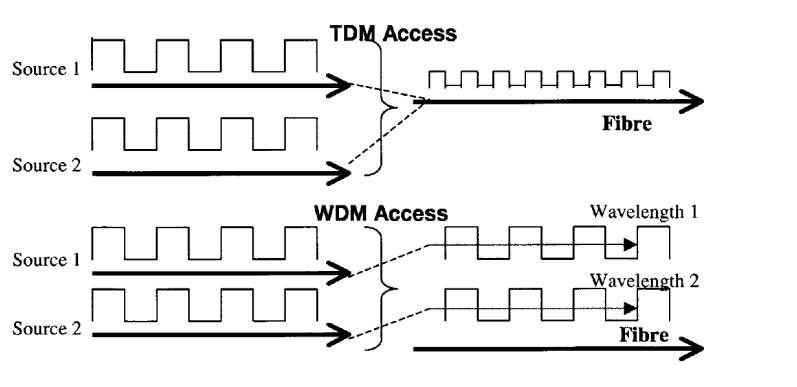
\includegraphics[width=0.8\textwidth]{snimky/TDMvsWDM.png}
    \label{fig:tdm-wdm}
\end{figure}

\subsection{Problematika přiřazení vlnových délek (RWA)}
Klasické datové sítě pracují s pakety, které jsou předávány mezi aktivními prvky. Výsledkem je přijetí paketu, kontrola cílové IP adresy a jeho následné odeslání přes zvolené rozhraní. Na druhou stranu optické sítě jsou data přenášená přes optické \enquote{crossconnect}, jenž každý přepíná optický signál, který je přenášen na různé vlnové délce do zvoleného směru.

Pro aplikaci ILP modelu uvažujme následující scénář:
\begin{itemize}
    \item Přiřazování vlnových délek je možné v rozdílných literaturách najít pod problematikou \enquote{barvení grafu}.
    \item Při přiřazování vlnových délek jsou optické trasy vytvářeny na požadavek, kdežto jejich cesty jsou dané předem (tedy fyzickými optickými vlákny mezi prvky)
    \item Pokud dvě trasy sdílí jedno optické vlákno, pak je ustanovena hrana mezi odpovídajícími uzly. V jiném případě nedojde k ustanovení hran, neboť neexistuje sdílené vlákno mezi trasou
    \item Jsou-li dva vrcholy připojeny k hranám, jedná se o sousedy. Vlnové délky odpovídají barvě v grafu
    \item Přiřazení barev v grafu musí splňovat základní podmínku, že stejná barva není přiřazena dvěma sousedícím vrcholům
\end{itemize}
